%!TEX root = SISC_elastic_3d.tex
\subsection{Semi-discretization of the elastic wave equation}\label{semi_discrete_form}

\begin{figure}[htbp]
	\centering
	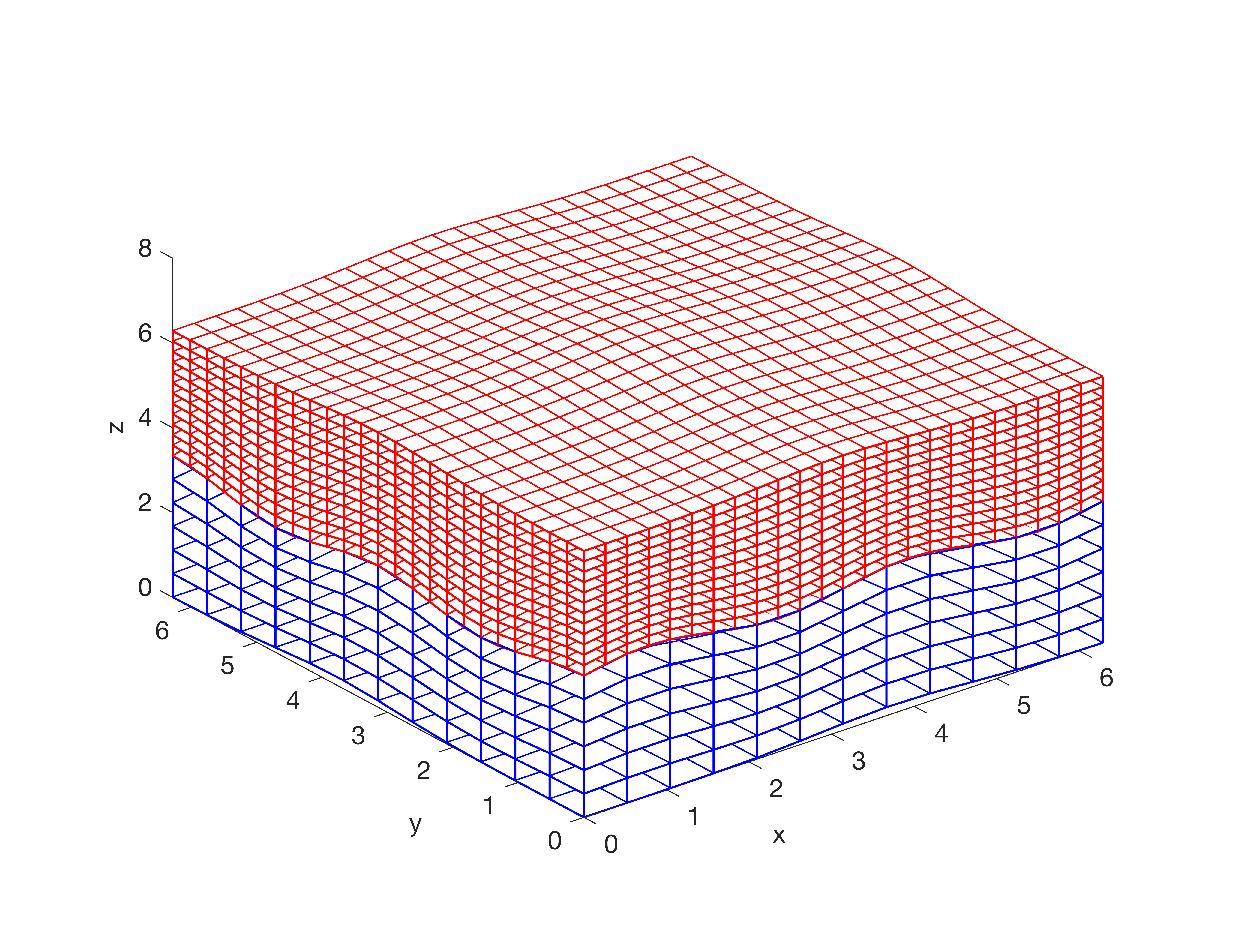
\includegraphics[width=0.6\textwidth,trim={0.4cm 0.7cm 0.8cm 1.4cm}, clip]{physical_discretization.eps}
	\caption{The sketch for the curvilinear mesh of the physical domain $\Omega$. The blue region is the spatial discretization of coarse subdomain $\Omega^c$ and the red region is the spatial discretization of the fine domain $\Omega^f$. Note that $x,y,z$ in the graph correspond to $x^{(1)}, x^{(2)}, x^{(3)}$ respectively. 
	 }\label{physical_discretization}
\end{figure}

In this section, we discretize the elastic wave equations (\ref{elastic_curvi}) and  (\ref{elastic_curvi_f}) with mesh refinement interface $\Gamma$. We assume the ratio of mesh sizes in the reference domains is $1:2$, that is the mesh sizes satisfy
\[h_1(n_1^h-1) = 1, \ \ \ h_2(n_2^h-1) = 1, \ \ \ h_3(n_3^h-1) = 1,\]
and
\[2h_1(n_1^{2h}-1) = 1, \ \ \ 2h_2(n_2^{2h}-1) = 1, \ \ \ 2h_3(n_3^{2h}-1) = 1.\]
 Other ratios can be treated analogously. Figure \ref{physical_discretization} gives an illustration of the discretization of a physical domain. This is an ideal mesh if the wave speed in $\Omega^f$ is half of the wave speed in $\Omega^c$.

In seismic wave simulation, far-field boundary conditions are often imposed in the $x^{(1)}$ and $x^{(2)}$ directions. Here, our focus is on the numerical treatment of the interface conditions (\ref{interface_cond}). Therefore, we assume periodic boundary conditions in $x^{(1)}$ and $x^{(2)}$ and ignore the boundaries in $x^{(3)}$. In Figure \ref{section_discretization}, we fix $x^{(2)} = 0$ and present the $x^{(1)}$-$x^{(3)}$ section of the domain $\Omega$ in both curvilinear space and parameter space.
\begin{figure}[htbp]
	\centering
	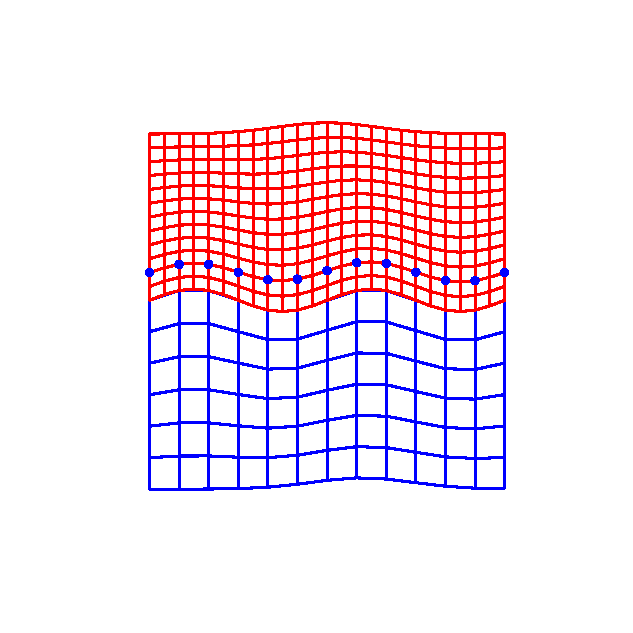
\includegraphics[width=0.45\textwidth,trim={1.0cm 2.0cm 1.0cm 1.8cm}, clip]{physical_section_discretization.eps}
	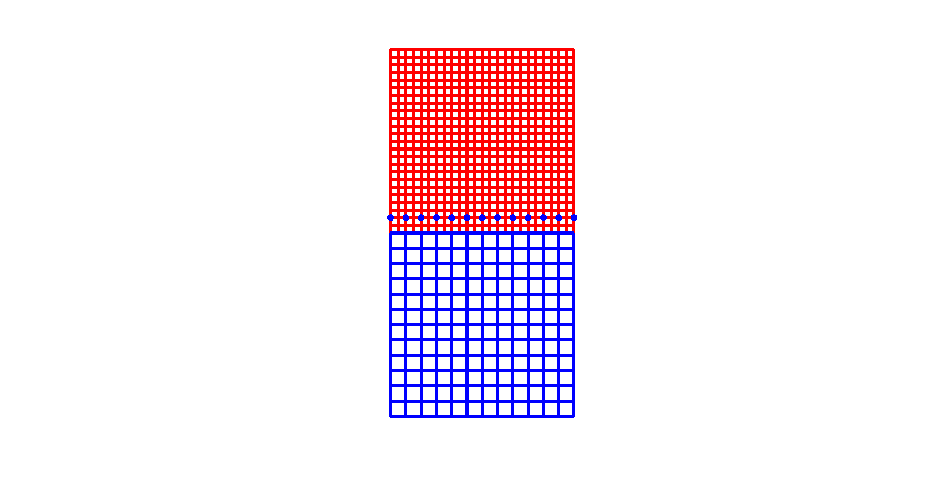
\includegraphics[width=0.45\textwidth,trim={1.0cm 2.0cm 1cm 1.8cm}, clip]{parameter_section_discretization.eps}
	%\caption{The sketch of spatial discretization of $x^{(1)}$-$x^{(3)}$ section with $x^{(2)} = 0$. From the left to the right are for physical domain and parameter space, respectively. The blue dots are the ghost points for the coarse domain $\Omega^c$.}\label{section_discretization}
\caption{The meshes in the physical domain (left) and parameter domain (right) of $x^{(1)}$-$x^{(3)}$ section with $x^{(2)} = 0$. The blue dots are the ghost points for the coarse domain $\Omega^c$.}\label{section_discretization}
\end{figure}
 To condense notations, we introduce the multi-index notations
\[{\bf i} = (i,j,k),\ \ {\bf r}_{\bf i} = (r^{(1)}_i,r^{(2)}_j,r^{(3)}_k),\ \ {\bf x}_{\bf i} = (x^{(1)}_i,x^{(2)}_j,x^{(3)}_k),\]
and group different sets of grid points according to
\begin{equation*}
\begin{aligned}
	I_{\Omega^c} &= \{i = 1,2,\cdots,n_1^{2h}, j = 1,2,\cdots,n_2^{2h}, k = 1,2,\cdots,n_3^{2h}\},\\
	I_{\Gamma^c} & = \{i = 1,2,\cdots,n_1^{2h}, j = 1,2,\cdots,n_2^{2h}, k = n_3^{2h}\},\\
	I_{\Omega^f} &= \{i = 1,2,\cdots,n_1^h, j = 1,2,\cdots,n_2^h, k = 1,2,\cdots,n_3^h\},\\
	I_{\Gamma^f} & = \{i = 1,2,\cdots,n_1^{h}, j = 1,2,\cdots,n_2^{h}, k = 1\}.
\end{aligned}	
\end{equation*}
The physical coordinates of the coarse grid points and fine grid points follow from the mappings ${\bf x}_{\bf i} = {\bf X}^c({\bf r}_{\bf i})$ and ${\bf x}_{\bf i} = {\bf X}^f({\bf r}_{\bf i})$, respectively. We denote a grid function by
\[{\bf u}_{\bf i} = {\bf u}_{i,j,k} = {\bf u}({\bf x}_{\bf i}),\]
where ${\bf u}$ can be either a scalar or vector. To distinguish between the continuous variables and the correspoding approximations on the grid, we use ${\bf c}_{\bf i}$ and ${\bf f}_{\bf i}$ to denote the grid functions for the approximations of ${\bf C}({\bf x}_{\bf i})$ and ${\bf F}({\bf x}_{\bf i})$, respectively. The components of $\bf c$ and $\bf f$ are ordered in the following way:\\
	%\begin{description}
		a). for each grid point ${\bf x}_{\bf i}$, there is a $3\times 1$ vector, say ${\bf c}_{\bf i} = (c^{(1)}_{\bf i}, c^{(2)}_{\bf i}, c^{(3)}_{\bf i})^T$ and ${\bf f}_{\bf i} = (f^{(1)}_{\bf i}, f^{(2)}_{\bf i}, f^{(3)}_{\bf i})^T$;\\
		b). the grid points are ordered such that they first loop over $r^{(1)}$ direction ($i$), then $r^{(2)}$ direction ($j$), and finally $r^{(3)}$ direction ($k$). More precisely, we have  
		${\bf c} = [c^{(1)}_{1,1,1}, c^{(2)}_{1,1,1}, c^{(3)}_{1,1,1},c^{(1)}_{2,1,1}, c^{(2)}_{2,1,1}, c^{(3)}_{2,1,1},\cdots]^T$ and ${\bf f} = [f^{(1)}_{1,1,1}, f^{(2)}_{1,1,1}, f^{(3)}_{1,1,1},f^{(1)}_{2,1,1}, f^{(2)}_{2,1,1}, f^{(3)}_{2,1,1},\cdots]^T$.
	%\end{description}
	
In the spatial discretization, we only use ghost points in the coarse domain and do not use ghost points in the fine domain. Comparing with the traditional approach of using ghost points in both domains, the system of linear equations at the interface becomes smaller and has a better structure. For the rest of the paper, the $\sim$ over an operator represents that the operator applies to a grid function with ghost points. We approximate the elastic wave equation (\ref{elastic_curvi}) in $\Omega^c$ by
\begin{equation}\label{elastic_semi_c}
{\rho}_{\bf i}^{c}\frac{d^2{{\bf c}_{\bf i}}}{dt^2} = \frac{1}{J^c_{\bf i}}\wt{\mathcal{L}}^{2h} {{\bf c}}_{\bf i},\quad {\bf i}\in I_{\Omega^c},\quad t>0.
\end{equation}
The discrete spatial operator is
\begin{equation}\label{L_operator}
\wt{\mathcal{L}}^{2h} {{\bf c}} = \left(\sum_{l=1}^2{Q}_l^{2h}({N}_{ll}^{2h}){\bf c}+\wt{{G}}_3^{2h}({N}_{33}^{2h}){{\bf c}}+\sum_{l=1}^3\sum_{m=1,m\neq l}^3{D}_l^{2h}({N}_{lm}^{2h}{D}_m^{2h}{\bf c})\right),
\end{equation}
and uses ghost points. % The term $Q_l^{2h}(N_{ll}^{2h}){\bf c}$ approximates $\bar{\partial}_l(N_{ll}\bar{\partial}_l{\bf C})$ are shown in Appendix \ref{appendix_cdomain}; $\wt{G}_3^{2h}(N_{33}^{2h}){\bf c}$ uses ghost points to approximate $\bar{\partial}_3(N_{33}\bar{\partial}_3 {\bf C})$ given in Appendix \ref{appendix_cdomain}; and $D_{l}^{2h}(N_{lm}^{2h}D_m^{2h}{\bf c})$ approximates $\bar{\partial}_l(N_{lm}\bar{\partial}_m {\bf C})$ are presented in Appendix \ref{appendix_cdomain}.
In Appendix \ref{appendix_cdomain}, the terms $Q_l^{2h}(N_{ll}^{2h}){\bf c}$, $\wt{G}_3^{2h}(N_{33}^{2h}){\bf c}$ and $D_{l}^{2h}(N_{lm}^{2h}D_m^{2h}{\bf c})$ are presented, which approximate $\bar{\partial}_l(N_{ll}\bar{\partial}_l{\bf C})$, $\bar{\partial}_3(N_{33}\bar{\partial}_3 {\bf C})$ and $\bar{\partial}_l(N_{lm}\bar{\partial}_m {\bf C})$, respectively.

Next, we approximate the elastic wave equation (\ref{elastic_curvi_f}) on the fine grid points. For all fine grid points that are not located at the interface $\Gamma$, the semi-discretization  is
\begin{equation}\label{elastic_semi_f}
{\rho}_{\bf i}^{f}\frac{d^2{{\bf f}_{\bf i}}}{dt^2} = \frac{1}{J^f_{\bf i}}{\mathcal{L}}^{h} {{\bf f}}_{\bf i},\quad {\bf i}\in I_{\Omega^f}\backslash I_{{\Gamma^f}},\quad t>0.
\end{equation}
Here, the discrete spatial operator is
\begin{equation}\label{Lf_operator}
{\mathcal{L}}^{h} {{\bf f}} = \left(\sum_{l=1}^2{Q}_l^{h}({N}_{ll}^h){\bf f}+{G}_3^{h}({N}_{33}^h){\bf f}+\sum_{l=1}^3\sum_{m=1,m\neq l}^3{D}_l^{h}({N}_{lm}^{h}{D}_m^{h}{\bf f})\right),
\end{equation}
which does not use any ghost points. The term ${G}_3^{h}(N_{33}^{h}){\bf f}$ approximating $\bar{\partial}_3(N_{33}\bar{\partial}_3 {\bf F})$ is presented in Appendix \ref{appendix_cdomain}; the terms $Q_l^{h}(N_{ll}^{h}){\bf f}$ and $D_{l}^{h}(N_{lm}^{2h}D_m^{h}{\bf f})$ approximate $\bar{\partial}_l(N_{ll}\bar{\partial}_l{\bf F})$ and $\bar{\partial}_l(N_{lm}\bar{\partial}_m {\bf F})$, respectively. Here, ${Q}_l^{h}({N}_{ll}^h){\bf f}$ and ${D}_l^{h}({N}_{lm}^{h}{D}_m^{h}{\bf f})$ are defined similar as those in (\ref{L_operator}), but with the grid points in $I_{\Omega^f}\backslash I_{{\Gamma^f}}$.

For the approximation at the interface $\Gamma$, we obtain the numerical solution by injection using a scaled interpolation operator
\begin{equation}\label{continuous_sol}
{\bf f}_{\bf i} = {\mathcal{P}}{\bf c}_{{\bf i}'},\quad {\bf i}\in I_{\Gamma^f},\quad {{\bf i}'}\in I_{\Gamma^c},
\end{equation}
which imposes the continuity of the solution at the interface $\Gamma$. 

For energy stability, the operator ${\mathcal{P}}$ must be in a specific form
%\[{\mathcal{P}} = (\mathcal{J}^h_\Gamma \bm{\Lambda}^h)^{-\frac{1}{2}}({\bf P}\otimes{\bf I})(\mathcal{J}^{2h}_\Gamma \bm{\Lambda}^{2h})^{\frac{1}{2}}.\]
\begin{equation}\label{scaleP}
{\mathcal{P}} = \left(({J}^h_\Gamma {\Lambda}^h)^{-\frac{1}{2}}{\bf P}({J}^{2h}_\Gamma {\Lambda}^{2h})^{\frac{1}{2}}\right)\otimes{\bf I}.
\end{equation}
Here, $J_{\Gamma}^h$ and $\Lambda^h$ are $n_1^{h}n_2^{h}\times n_1^{h}n_2^{h}$ diagonal matrices. The diagonal elements of $J_{\Gamma}^h$ and $\Lambda^{h}$ are $J^f$ and $|\nabla_x R^{f,(3)}|$ evaluated at fine grid points in $I_{\Gamma^f}$, respectively. Similarly, ${J}_{\Gamma}^{2h}$ and ${{\Lambda}^{2h}}$ are $n_1^{2h}n_2^{2h}\times n_1^{2h}n_2^{2h}$ diagonal matrices. The diagonal elements of $J_{\Gamma}^{2h}$ and $\Lambda^{2h}$ are $J^c$ and $|\nabla_x R^{c,(3)}|$ evaluated at coarse grid points in $I_{\Gamma^c}$, respectively. Because the spatial dimension of the governing equation is 3, the matrix ${\bf I}$ is a $3\times 3$ identity matrix. Finally, ${\bf P}$ is an interpolation operator of size $n_1^hn_2^h\times n_1^{2h}n_2^{2h}$ for scalar grid functions at $\Gamma^c$. Since the spatial discretization is fourth order accurate, we also use a fourth order interpolation. With mesh refinement ratio  $1:2$, the stencils ${\bf P}$ have four cases as illustrated in  Figure \ref{interpolation}. Consequently, the scaled interpolation operator $\mathcal{P}$ is also fourth order accurate.

In computer implementation, we use \eqref{continuous_sol} to obtain the solution at the interface of the fine domain. However, in the energy analysis in  Sec.~\ref{sec_energy}, it is more convenient to use the equivalent form
%We note that \eqref{continuous_sol} is equivalent to 
\begin{equation}\label{elastic_semi_f_i}
{\rho}^f_{\bf i} \frac{d^2{\bf f}_{\bf i}}{dt^2} =
\frac{1}{J^f_{\bf i}}(\mathcal{L}^h{\bf f}_{\bf i} + {\bm \eta}_{\bf i}), \quad {\bf i}\in I_{\Gamma^f}
\end{equation}
with 
\begin{equation}\label{eta}
{\bm \eta}_{\bf i} = {\rho}^f_{\bf i}J^f_{\bf i}{\mathcal{P}}\left(\frac{1}{\rho^c_{{\bf i}'}J^c_{{\bf i}'}}\wt{\mathcal{L}}^{2h} {\bf c}_{{\bf i}'}\right) - \mathcal{L}^{h}{\bf f}_{\bf i}, \quad {\bf i}\in I_{\Gamma^f},\quad {{\bf i}'}\in I_{\Gamma^c}.
\end{equation}
%which is useful in the energy analysis in the next section. 
The variable $\bm \eta$ in (\ref{eta}) is approximately zero with a second order truncation error, which is of the same order as the boundary stencil of the SBP operator. Hence,  $\bm \eta$ does not affect the order of truncation error in the spatial discretization. %Therefore, it does not affect the overall accuracy of the semi-discretization. 
For the simplicity of analysis, we introduce a general notation for the schemes (\ref{elastic_semi_f}) and (\ref{elastic_semi_f_i}) in the fine domain $\Omega^f$,
\begin{align}\label{fine_scheme}
{\rho}^f_{\bf i}\frac{d^2{\bf f}_{\bf i}}{dt^2} =\frac{1}{J^f_{\bf i}}\hat{\mathcal{L}}^h{\bf f}_{\bf i} = \left\{
\begin{aligned}
&\frac{1}{J^f_{\bf i}}(\mathcal{L}^h{\bf f}_{\bf i} +{\bm \eta}_{\bf i}), \quad {\bf i}\in I_{\Gamma^f}\\
&\frac{1}{J^f_{\bf i}}\mathcal{L}^h{\bf f}_{\bf i},\quad\quad\quad {\bf i}\in I_{\Omega^f}\backslash I_{\Gamma^f} 
\end{aligned}
\right. \quad t > 0.
\end{align}
%In computer implementation, we use \eqref{continuous_sol} to obtain the solution at the interface of the fine domain. The reason for introducing \eqref{elastic_semi_f_i} is that it will be helpful in the energy analysis in Sec.~\ref{sec_energy}.

The following condition imposes continuity of traction at the interface, the first equation in (\ref{interface_cond}),
\begin{equation}\label{continuous_traction}
(\Lambda^{c}_{{\bf i}'}J_{{\bf i}'}^{c})^{-1}\wt{\mathcal{A}}_3^{2h}{\bf c}_{{\bf i}'}
= {\mathcal{R}}\Big((\Lambda^f_{\bf i}{ J}^f_{\bf i})^{-1}(\mathcal{A}_3^h{\bf f}_{\bf i}-h_3\omega_1{\bm \eta}_{\bf i})\Big), \quad {\bf i}\in I_{\Gamma^f},\quad {{\bf i}'}\in I_{\Gamma^c}.
\end{equation}
Here, $(\Lambda^{c}_{{\bf i}'}J_{{\bf i}'}^{c})^{-1}\wt{\mathcal{A}}_3^{2h}{\bf c}_{{\bf i}'}$ approximates the traction, $\frac{A_3^c\nabla_r{\bf C}}{J^c\left|\nabla_x R^{c,(3)}\right|}$, at the interface of the coarse domain with $\Lambda_{{\bf i}'}^c = |\nabla_x R^{c,(3)}({\bf x}_{{\bf i}'})|$ and
\begin{equation}\label{hatAc}
\wt{\mathcal{A}}_3^{2h}{\bf c} = {N}_{31}^{2h}{D}^{2h}_1{\bf c} + {N}_{32}^{2h}{D}^{2h}_2{\bf c} + {N}_{33}^{2h}\wt{\mathcal{D}}^{2h}_3{\bf c},
\end{equation}
where ${N}_{3l}^{2h}D_l^h{\bf c}$ approximates $N_{3l}\bar{\partial}_l{\bf C}$ and ${N}_{33}^{2h}\wt{\mathcal{D}}_3^{2h}{\bf c}$ approximates $N_{33}\bar{\partial}_3{\bf C}$ are given in Appendix \ref{appendix_cdomain}; $(\Lambda^f_{\bf i}{ J}^f_{\bf i})^{-1}\mathcal{A}_3^h{\bf f}_{\bf i}$ approximates the traction, $\frac{A_3^f\nabla_r{\bf F}}{J^f\left|\nabla_x R^{f,(3)}\right|}$, at the interface of the fine domain with $\Lambda_{\bf i}^f = |\nabla_x R^{f,(3)}({\bf x}_{\bf i})|$ and 
\begin{equation}\label{hatAf}
\mathcal{A}_3^h{\bf f} = {N}_{31}^{h}{D}^h_1{\bf f} + {N}_{32}^h{D}^h_2{\bf f} + {N}_{33}^h\mathcal{D}_3^h{\bf f},
\end{equation}
where ${N}_{3l}^{h}D_l^{h}{\bf f}$ approximating $N_{3l}\bar{\partial}_l{\bf F}$ have similar definitions as those in (\ref{hatAc}), but correspond to the grid points in $I_{\Gamma^f}$, ${N}_{33}^{2h}{\mathcal{D}}^{2h}_3{\bf f}$ approximating $N_{33}\bar{\partial}_3{\bf F}$ is given in Appendix \ref{appendix_cdomain}; the term $h_3\omega_1{\bm \eta}_{\bf i}$ originates from the fact that ghost points are only used in the coarse domain but not in the fine domain. The term is important for energy stability, as shown in Theorem \ref{thm1}. It is a penalty term on the order of the truncation error and thus (\ref{continuous_traction})  provides a valid way of enforcing the continuity of traction at the interface, $\omega_1$ is a weight in the inner product (\ref{inner_product}); $\mathcal{R}$ is a scaled restriction operator with the structure 
\begin{equation}\label{scaleR}
 {\mathcal{R}} =  \left(({J}^{2h}_\Gamma{\Lambda}^{2h})^{-\frac{1}{2}}{\bf R}({J}^{h}_\Gamma {\Lambda}^h)^{\frac{1}{2}}\right)\otimes {\bf I},
 \end{equation}
 where ${\bf R}$ is a restriction operator of size $n_1^{2h}n_2^{2h}\times n_1^hn_2^h$ for scalar grid funcitons. It is determined by the compatibility condition ${\bf R}=\frac{1}{4}{\bf P}^T$, see the stencils in Figure \ref{restriction}. As will be seen later, the compatibility condition, as well as the scaling of the interpolation and restrictions, are essential for energy stability \cite{Lundquist2018}. We want to remark that the condition \eqref{continuous_traction} determines the ghost points values in the coarse domain. 
 
Let ${\bf u}$ and ${\bf v}$ be grid functions in coarse domain $\Omega^c$, we define the discrete inner product at the interface by
\begin{equation}\label{scalar_product_discrete_interface_c}
\left<{\bf u}, {\bf v}\right>_{2h} = 4h_1h_2\sum_{i=1}^{n_1^{2h}}\sum_{j=1}^{n_2^{2h}}{  J}_{i,j,n_3^{2h}}^{c}\Lambda^{c}_{i,j,n_3^{2h}}({\bf u}_{i,j,n_3^{2h}}\cdot {\bf v}_{i,j,n_3^{2h}}).
\end{equation}
Similarly, the discrete inner product at the interface for fine domain $\Omega^f$ is defined as
\begin{equation}\label{scalar_product_discrete_interface_f}
\left<{\bf u}, {\bf v}\right>_{h} = h_1h_2\sum_{i=1}^{n_1^{h}}\sum_{j=1}^{n_2^{h}}{  J}_{i,j,1}^{f}\Lambda^{f}_{i,j,1}({\bf u}_{i,j,1}\cdot {\bf v}_{i,j,1})
\end{equation}
with $\bf u$ and $\bf v$ are grid functions in fine domain $\Omega^f$. Then we have the following lemma.
 
 \begin{lemma}\label{lemma1}
 	Let ${\bf c}$ and ${\bf f}$ be grid functions at the interface for coarse domain and fine domain, respectively. Then the interpolation operator $\mathcal{P}$ and the restriction operator $\mathcal{R}$ satisfy
 	\begin{equation}\label{pr_relation}
 	\left<\mathcal{P} {\bf c}, {\bf f}\right>_h = \left<{\bf c}, \mathcal{R}{\bf f}\right>_{2h}
 	\end{equation}
 	if $\bm{R} = \frac{1}{4}\bm{P}^T$. 
 \end{lemma}
 \begin{proof}
 	%Since 
 	%\begin{align*}
 	%{\mathcal{P}} &= (\mathcal{J}^h_\Gamma \bm{\Lambda}^h)^{-\frac{1}{2}}({\bf P}\otimes{\bf I})(\mathcal{J}^{2h}_\Gamma \bm{\Lambda}^{2h})^{\frac{1}{2}}\\
 	%& = ((J_{\Gamma}^h\otimes{\bf I})(\Lambda^h\otimes{\bf I}))^{-\frac{1}{2}}({\bf P}\otimes{\bf I})((J_{\Gamma}^{2h}\otimes{\bf I})(\Lambda^{2h}\otimes{\bf I}))^{\frac{1}{2}}\\
 	%& = (J_{\Gamma}^h\Lambda^h)^{-\frac{1}{2}}{\bf P}(J_{\Gamma}^{2h}\Lambda^{2h})^{\frac{1}{2}}\otimes{\bf I},
 	%\end{align*}
 	%and
 	%\begin{align*}
 	%{\mathcal{R}} &= (\mathcal{J}^{2h}_\Gamma \bm{\Lambda}^{2h})^{-\frac{1}{2}}({\bf R}\otimes{\bf I})(\mathcal{J}^{h}_\Gamma \bm{\Lambda}^{h})^{\frac{1}{2}}\\
 	%& = ((J_{\Gamma}^{2h}\otimes{\bf I})(\Lambda^{2h}\otimes{\bf I}))^{-\frac{1}{2}}({\bf R}\otimes{\bf I})((J_{\Gamma}^{h}\otimes{\bf I})(\Lambda^{h}\otimes{\bf I}))^{\frac{1}{2}}\\
 	%& = (J_{\Gamma}^{2h}\Lambda^{2h})^{-\frac{1}{2}}{\bf R}(J_{\Gamma}^{h}\Lambda^{h})^{\frac{1}{2}}\otimes{\bf I},
 	%\end{align*}
 	%then
 	From \eqref{scalar_product_discrete_interface_c}--\eqref{scalar_product_discrete_interface_f}, the definiton of $\mathcal{P}$ in \eqref{scaleP} and $\mathcal{R}$ in \eqref{scaleR}, we obtain
 	\begin{align*}
 	\left<\mathcal{P}{\bf c}, {\bf f}\right>_h &= h_1h_2\left[\left((J_{\Gamma}^h\Lambda^h)^{\frac{1}{2}} {\bf P}(J_{\Gamma}^{2h}\Lambda^{2h})^{\frac{1}{2}}\otimes {\bf I}\right){\bf c}\right]^T\cdot{\bf f}\\
 	& = 4h_1h_2 {\bf c}^T \cdot \left[\left((J_{\Gamma}^{2h}\Lambda^{2h})^{\frac{1}{2}}\frac{1}{4}{\bf P}^T(J_{\Gamma}^h\Lambda^h)^{\frac{1}{2}}\otimes {\bf I}\right) {\bf f}\right]\\
 	& =4h_1h_2 {\bf c}^T \cdot \left[\left((J_{\Gamma}^{2h}\Lambda^{2h})^{\frac{1}{2}}{\bf R}(J_{\Gamma}^h\Lambda^h)^{\frac{1}{2}}\otimes {\bf I}\right) {\bf f}\right] = \left<{\bf c}, \mathcal{R}{\bf f}\right>_{2h}
 	\end{align*}
 \end{proof}
 

\begin{figure}%[htbp]
	\centering
	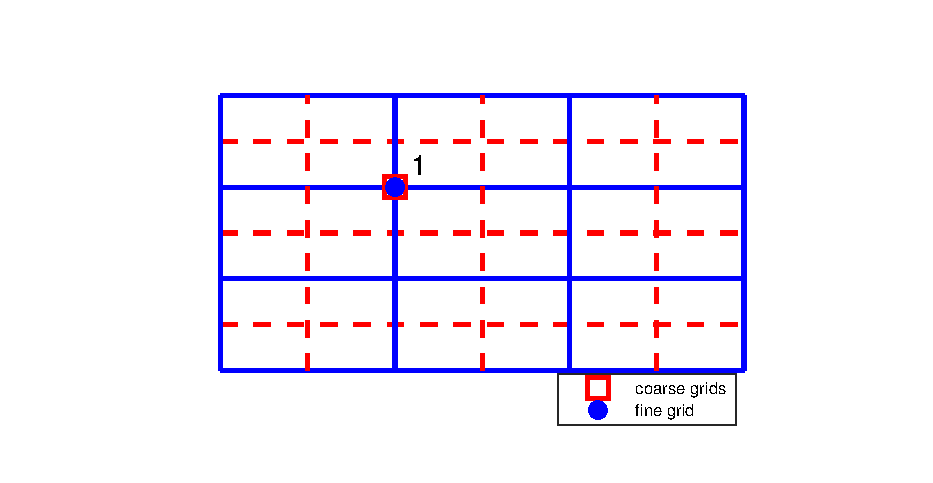
\includegraphics[width=0.24\textwidth,trim={1.8cm 0.8cm 1.4cm 1.2cm}, clip]{interpolation1.eps}
	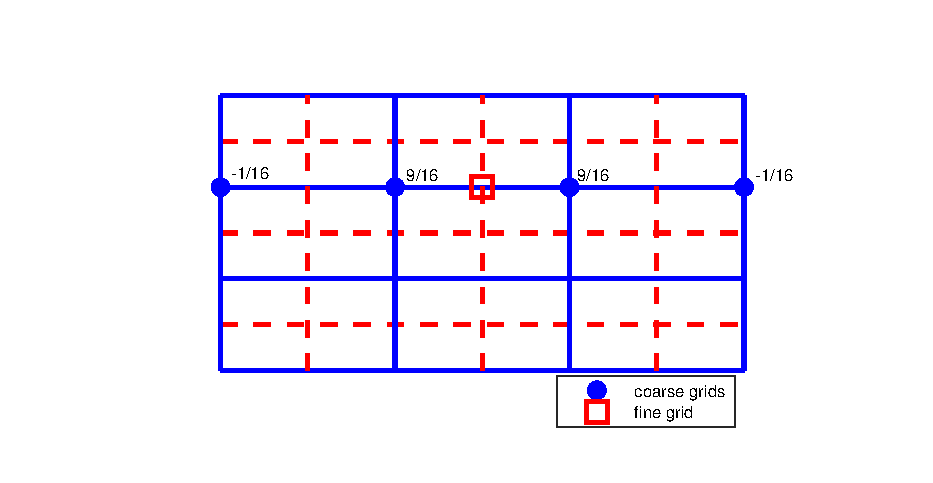
\includegraphics[width=0.24\textwidth,trim={1.8cm 0.8cm 1.4cm 1.2cm}, clip]{interpolation2.eps}
	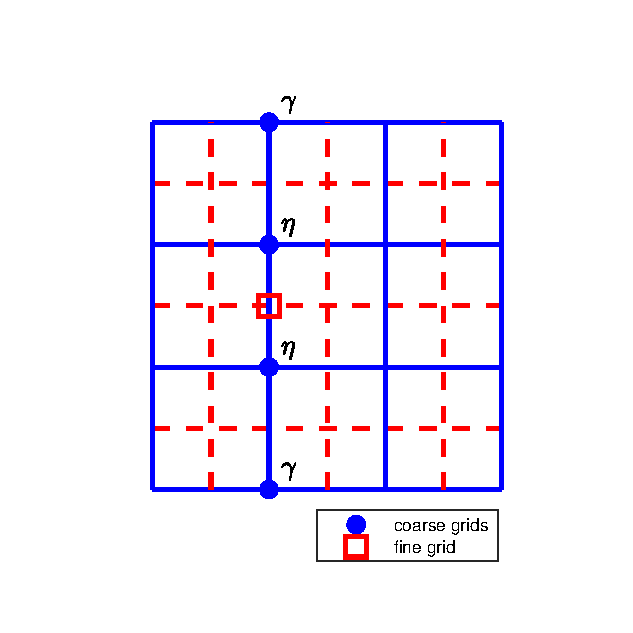
\includegraphics[width=0.24\textwidth,trim={1.8cm 0.8cm 1.4cm 1.2cm}, clip]{interpolation3.eps}
	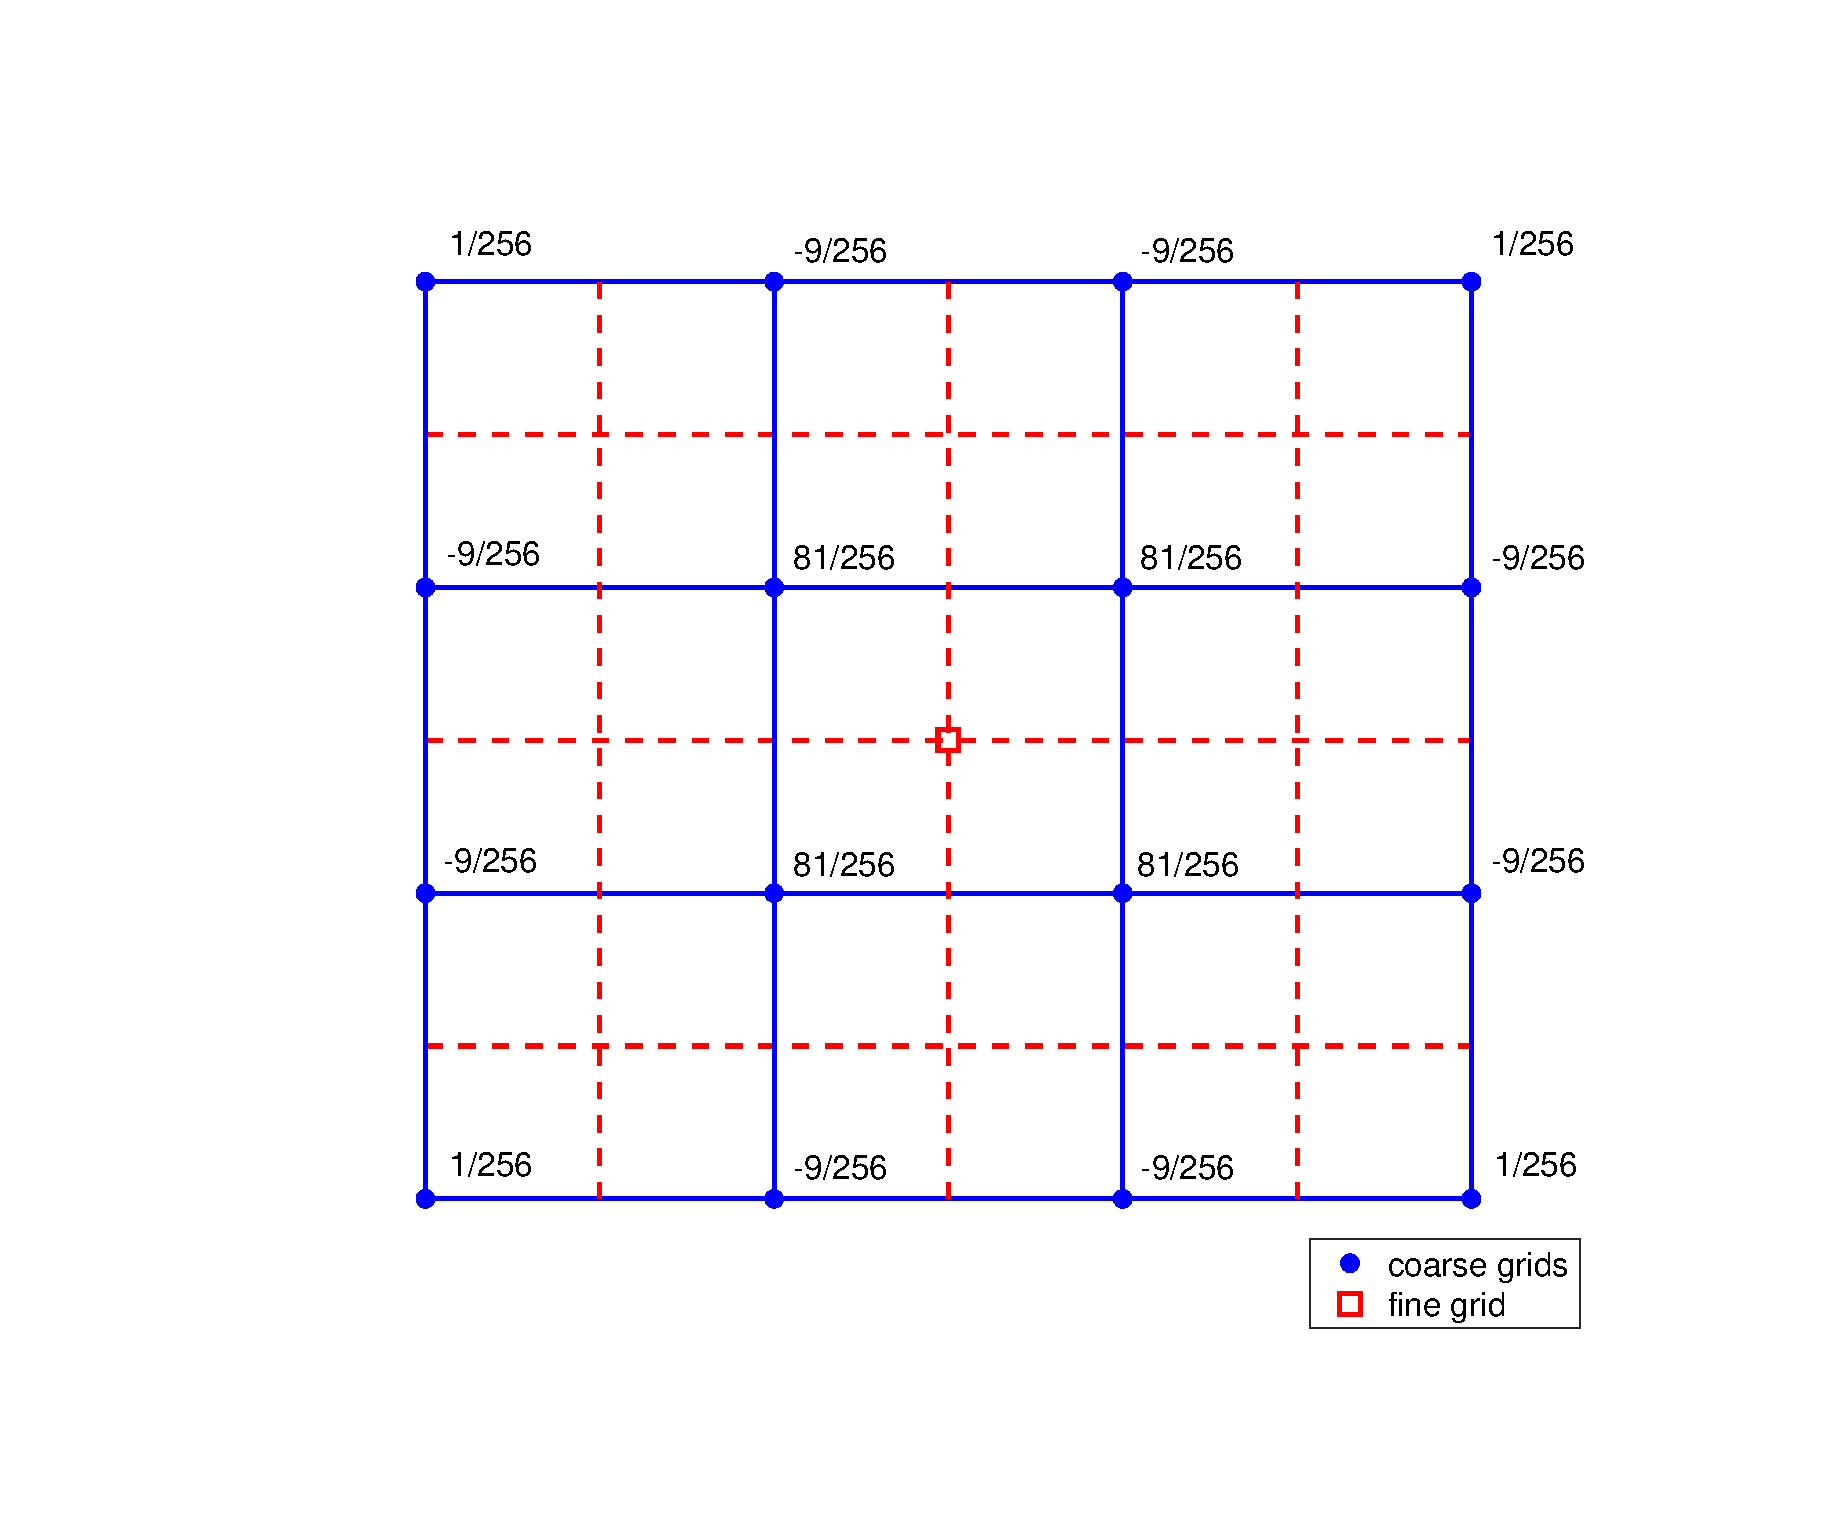
\includegraphics[width=0.24\textwidth,trim={1.8cm 0.8cm 1.4cm 1.2cm}, clip]{interpolation4.eps}
	\caption{The sketch for the stencils of fourth order interpolation operator ${\bf P}$ in two dimensions with parameters $\gamma = -\frac{1}{16}$, $\eta = \frac{9}{16}$, $\mu = 1$, $\alpha = \frac{1}{256}$, $\beta = -\frac{9}{256}$ and $\theta = \frac{81}{256}$. }\label{interpolation}
\end{figure}
\begin{figure}[htbp]
	\centering
	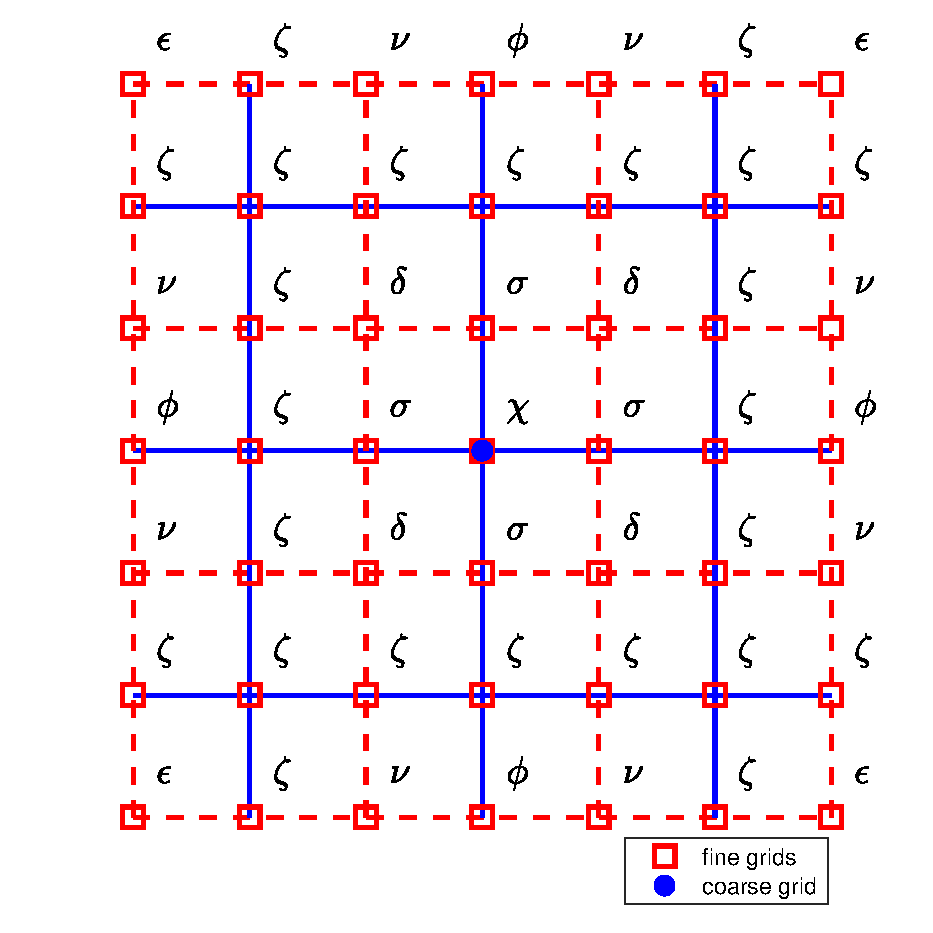
\includegraphics[width=0.6\textwidth]{restriction.eps}
	\caption{The sketch for the stencil of fourth order restriction operator ${\bf R}$ in two dimensions with parameters $\epsilon = \frac{1}{1024}$, $\nu = -\frac{9}{1024}$, $\phi = -\frac{16}{1024}$, $\delta = \frac{81}{1024}$, $\sigma = \frac{144}{1024}$, $\chi = \frac{256}{1024}$ and $\zeta = 0$.}\label{restriction}
\end{figure}




